\documentclass[user_manual.tex]{subfiles}
\begin{document}
 
 \chapter{Software}

\begin{itemize}
	\item{AI (VIRBOT)}

	\item{Navegación}
	
	\item{Visión}
	
	\item{Habla}
\end{itemize}

\section{VIRBOT}

El sistema VIRBOT consiste de varios subsistemas los cuales controlan la operación del robot móvil.


\section{Guia principal para el desarrollo de codigo}
\begin{itemize}
 \item Todo código fuente DEBE estar contenido en la carpeta \textit{catkin\_ws/src}.\\
 
 \item Sólo el código contenido en la carpeta catkin\_ws/src/hardware puede interactuar con el 
 harware del robot\\
 
 \item El punto anterior implica que todos los otros programas deberán implementar SÓLO algoritmos. 
 Todas las interacciones con el hardware (e.g.. obtener una imagen desde la cámara, leer el láser, 
 mover la base o la cabeza, hablar, etc.) debe hacerse intercambiando información con los paquetes
 contenidos en la carpeta \textbf{hardware}, a través de los tópicos y servicios de ROS.
 
 \item Los códigos contenidos en todas las carpetas dentro de \textit{catkin\_ws/src}, excepto las carpetas de 
 herramientas, DEBEN contener sólo código escrito por el propio desarrollador (de cualquier paquete).
 Todas las bibliotecas necesarias o código de otras fuentes (bibliotecas serial, arduino, julius,
 dynamixel, etc.), si no están instaladas en algún default path (/opt/ros, /usr/local/, etc.), deben 
 ser puestas dentro de la carpeta \textit{catkin\_ws/src/tools} en una sub-carpeta apropiada.\\
 
 \item Los desarrolladores deben tratar de usar sólo mensajes ya definidos en algún paquete de ROS o
 pila, sin embargo, si mensajes personalizados son requeridos, éstos deben ser puestos dentro de
 \textit{catkin\_ws/src/subsystem/subsystem\_maga}, así que, muchos mensajes pueden ser usados sin necesidad
 de ejecutar todos los demás subsistemas.\\
\end{itemize}


\section{Estructura de la carpeta}
\begin{verbatim}
catkin_ws
  build
  devel
  src
      hardware
	  arms
	  battery
	  hardware_state
	  justina_urdf
	  hardware_msgs
	  head
	  mobile_base
	  point_cloud_manager
	  speakers
	  torso
      hri
	  gesture_recog
	  hri_msgs
	  justina_gui
	  natural_language
	  speech_recog
      interoperation
	  bbros_bridge
	  joy_teleop
	  pc_teleop
	  roah_rsbb
      manipulation
	  arms_predef_movs
	  arms_path_planning
	  arms_trajectory_planning
	  head_predef_movs
	  head_tracking_point
	  manipulation_msgs
      navigation
	  localization
	  mapping
	  moving
	  navigation_msgs
	  path_planning
	  point_traking
      planning
	  planning_msgs
	  pomdp
	  rule_based
	  semantic_database
	  state_machines
      surge_et_ambula
	  launch
	  rviz_files
      testing
	  any_not_stable_node
      tools
	  ros_tools
	  libraries
	      serial_arduino
	      serial_dynamixel
	      julius
	      festival
      vision
	  door_detector
	  furniture_recog
	  object_detector
	  object_recog
	  person_detection
	  person_recog
	  vision_msgs
user_manual
\end{verbatim}
%\chapter{Ayuda y referencias}
Cada paquete en la carpeta de \textit{hardware} debe tener su versión simulada, así que, el resto del 
software (todas las otras carpetas se supone que contienen sólo algoritmos y no interacción con el 
hardware del robot) puedes correr inmediatamente el modo de simulación. Eligiendo entre simulado o 
real debe ser hecho en la carpeta de ejecución.


\section{Nodos de ROS}
Con el comando \textit{rosrun} se puede ejecutar un nodo de un paquete sin tener que conocer la ruta completa, indicando el nombre del paquete dentro del cual se encuentra el nodo que deseamos lanzar y el nombre del ejecutable.\\

Uso:\\\\
%\fbox{\parbox[b]{\linewidth}{\texttt{\$ rosrun package\_name executable\_name}}}\\
\begin{minted}[
frame=lines,
framesep=1mm,
bgcolor=black,
baselinestretch=1.2
]{console}
 rosrun package_name executable_name
\end{minted}

Por otro lado, \textit{roslaunch} es una herramienta para lanzar fácilmente múltiples nodos de ROS de forma local y remota a través de SSH, así como establecer parámetros en el Servidor de Parámetros. Antes de iniciar cualquier nodo, \textit{roslaunch} determinará si \textit{roscore} ya está en ejecución y, en caso contrario, lo iniciara automáticamente. Los archivos \textit{.launch} del robot Justina se encuentran dentro del paquete \textit{surge\_et\_ambula} en la carpeta \textit{launch}.\\

Uso:\\\\
%\fbox{\parbox[b]{\linewidth}{\texttt{\$ roslaunch package\_name file\_name.launch}}}\\
\begin{minted}[
frame=lines,
framesep=1mm,
bgcolor=black,
baselinestretch=1.2
]{console}
 roslaunch package_name file_name.launch
\end{minted}

Los archivos \textit{launch} son documentos XML, y cada documento XML debe tener un elemento raíz, para el caso de los archivos \textit{launch} de ROS, el elemento raíz se define mediante un par de etiquetas \texttt{launch}:

\begin{minted}[
frame=lines,
framesep=1mm,
baselinestretch=1.2
]{xml}
<launch>
</launch>
\end{minted}

Todos los demás elementos del archivo se deben incluir dentro de estas etiquetas.\\

La etiqueta \texttt{$ < $node$ > $} especifica un nodo ROS que se desea lanzar y tiene tres atributos requeridos, ésta etiqueta se ve de esta forma:

\begin{minted}[
frame=lines,
framesep=1mm,
baselinestretch=1.2
]{xml}
<node name="node-name" pkg="package-name" type="executable-name" />
\end{minted}

Los atributos \texttt{pkg} y \texttt{type} identifican qué programa debe ejecutar ROS para iniciar este nodo. Estos son los mismos dos argumentos que toma el comando \textit{rosrun}, especificando el nombre del paquete y el nombre del ejecutable, respectivamente. El atributo \texttt{name} asigna un nombre al nodo. Esto anula cualquier nombre que el nodo se asignaría normalmente a sí mismo en su llamada a \texttt{ros::init}.\\

Existen otros atributos opcionales utilizados en la etiqueta \texttt{$ < $node$ > $}:
\begin{itemize}
\item \texttt{args=``arg1 arg2 arg3''}: Pasar argumentos al nodo.
\item \texttt{output=``screen''}: Los nodos iniciados con este atributo mostrarán sus salidas stdout/stderr  en la pantalla.
\end{itemize}
 
%La barra inclinada cerca del final de la etiqueta del nodo es importante y fácil de olvidar. Indica que no hay ninguna etiqueta de cierre ("</ node>") y que el elemento de nodo está completo.

La etiqueta \texttt{$ < $group$ > $} facilita la aplicación de configuraciones a un grupo de nodos. Tiene un atributo \texttt{ns} que le permite definir un \textit{namespace} independiente para un grupo de nodos.

\begin{minted}[
frame=lines,
framesep=1mm,
baselinestretch=1.2
]{xml}
<group ns="namespace">
	<node name="node-name" pkg="package-name" type="executable-name" />
</group>
\end{minted}

La etiqueta \texttt{$ < $group$ > $} es equivalente a la etiqueta de nivel superior \texttt{$ < $launch$ > $} y simplemente actúa como un contenedor para las etiquetas que se encuentran dentro. Esto significa que puede usar cualquier etiqueta como se usaría normalmente dentro de una etiqueta \texttt{$ < $launch$ > $}.\\

Los nodos de ROS también admiten reasignaciones, que proporcionan un nivel de control para modificar los nombres utilizados por los nodos. Las reasignaciones se basan en la idea de sustitución: cada reasignación proporciona un nombre original y un nuevo nombre. Para reasignar nombres dentro de un archivo \textit{launch} se utiliza la etiqueta \texttt{$ < $remap$ > $}:

\begin{minted}[
frame=lines,
framesep=1mm,
baselinestretch=1.2
]{xml}
<remap from="original-name" to="new-name"/>
\end{minted}

Si la etiqueta \texttt{$ < $remap$ > $} aparece en el nivel superior como hijo de la etiqueta \texttt{$ < $launch$ > $}, esta reasignación se aplicará a todos los nodos subsiguientes. Estos elementos de reasignación también pueden aparecer como hijos de una etiqueta \texttt{$ < $node$ > $}, en este caso, los reasignamientos dados se aplican solamente al nodo en el que estén contenidos, como en este ejemplo:

\begin{minted}[
frame=lines,
framesep=1mm,
baselinestretch=1.2
]{xml}
<node name="node-name" pkg="package-name" type="executable-name" >
	<remap from="original-name" to="new-name" />
</node>
\end{minted}

La etiqueta \texttt{$ < $param$ > $} define un parámetro que se establecerá en el Servidor de Parámetros. Esta etiqueta, como uno habría de esperar, asigna el valor dado al parámetro con el nombre dado.

\begin{minted}[
frame=lines,
framesep=1mm,
baselinestretch=1.2
]{xml}
<param name="param-name" value="param-value" />
\end{minted}

La etiqueta \texttt{$ < $param$ > $} se puede colocar dentro de una etiqueta \texttt{$ < $node$ > $}, en cuyo caso el parámetro se trata como un parámetro privado.

\begin{minted}[
frame=lines,
framesep=1mm,
baselinestretch=1.2
]{xml}
<node name="node-name" pkg="package-name" type="executable-name" >
	<param name="param-name" value="param-value" />
</node>
\end{minted}

Para obtener más información acerca de estas etiquetas y de los archivos \textit{launch}, por favor consulte: \url{http://wiki.ros.org/roslaunch/XML}. 
%*************************************************************************************
%*************************************************************************************

\subsection{Nodo /robot\_state\_publisher}
Este nodo se encuentra dentro del paquete \textit{robot\_state\_publisher}, y permite publicar el estado del robot a \textit{tf}. Una vez que el estado se publica, está disponible para todos los componentes del sistema que utlizan \textit{tf}. El paquete toma las posiciones de las juntas del robot como entrada y publica las poses 3D de los eslabones usando un modelo de árbol cinemático. \textit{tf} es un paquete que permite al usuario realizar el seguimiento de varios marcos de referencia a lo largo del tiempo.\\

\textit{robot\_state\_publisher} usa el URDF especificado por el parámetro \textit{robot\_description}, y las posiciones de las juntas del tópico \textit{joint\_states} para calcular la cinemática directa del robot y publicar los resultados a través de \textit{tf}. URDF (Unified Robot Description Format) es un formato  XML para representar el modelo de un robot.

%Principio de la tabla
\begin{table}[H]
\begin{center}
\begin{tabular}{|l|l|p{4cm}|}%Define el número de columnas
\hline

Tópicos suscritos &  /joint\_states [sensor\_msgs/JointState] & Se suscribe a la información de la posición de las juntas \\ 
& & \\
\hline

Tópicos publicados &  /tf [tf/tfMessage] & Publica el estado del robot \\
& & \\
\hline

\multirow{4}{*}{Parámetros} 
&  robot\_description [urdf map, default: ] & Archivo XML del modelo del robot \\
& & \\
& tf\_prefix [string, default: ]  & Establece el prefijo tf para el namespace\\
& & \\
& publish\_frequency [double, default: 50Hz] & Frecuencia a la que publica el nodo\\
& & \\
& use\_tf\_static [bool, default: false]  & Define si se quiere utilizar /tf\_static\\
\cline{1-3}

\end{tabular}
\caption{Nodo /robot\_state\_publisher}
\label{robot state publisher node}
\end{center}
\end{table}
%Fin de la tabla

%\textbf{Ajuste de parámetros}\\
\textbf{Sintaxis en un archivo launch}\\
Lanzamiento del nodo y ajuste del parámetro \textit{robot\_description}.
\begin{minted}[
frame=lines,
framesep=1mm,
baselinestretch=1.2
]{xml}
<param name="robot_description" command="cat $(find knowledge)/hardware/justina.xml"/>
<node name="robot_state_publisher" pkg="robot_state_publisher" type="state_publisher"/>$
\end{minted}
%\fbox{\parbox[b]{\linewidth}{ \texttt{$<$param name=``robot\_description'' command=``cat \$(find knowledge)/hardware/justina.xml''/$>$\\
%$<$node name=``robot\_state\_publisher'' pkg=``robot\_state\_publisher'' type=``state\_publisher''/$>$}}}\\

En el archivo \textit{justina.xml} se encuentra el modelo del robot Justina; en la Figura  \ref{fig:Sofware:Arbol} se tiene el árbol de transformaciones, los ovalos azules representan las juntas, mientras que los recuadros negros representan los sistemas de referencia asociados a los eslabones del robot. En el grafo dirigido se muestran los offset de traslación en \textit{x}, \textit{y} y \textit{z}, y los offset de los ángulos de rotación \textit{roll}, \textit{pitch} y \textit{yaw} que se tienen entre los sistemas de referencia, las unidades están en metros y radianes respectivamente.\\

En el grafo dirigido de la Figura \ref{fig:Sofware:Frames} se muestran todas las transformaciones entre sistemas de referencia para el robot, en éste grafo se incluyen además los marcos \textit{odom} y \textit{map}. Para más información acerca de los sistemas de referencia para plataformas móviles consulte: \url{http://www.ros.org/reps/rep-0105.html}.

\begin{figure}[H]
\begin{center}
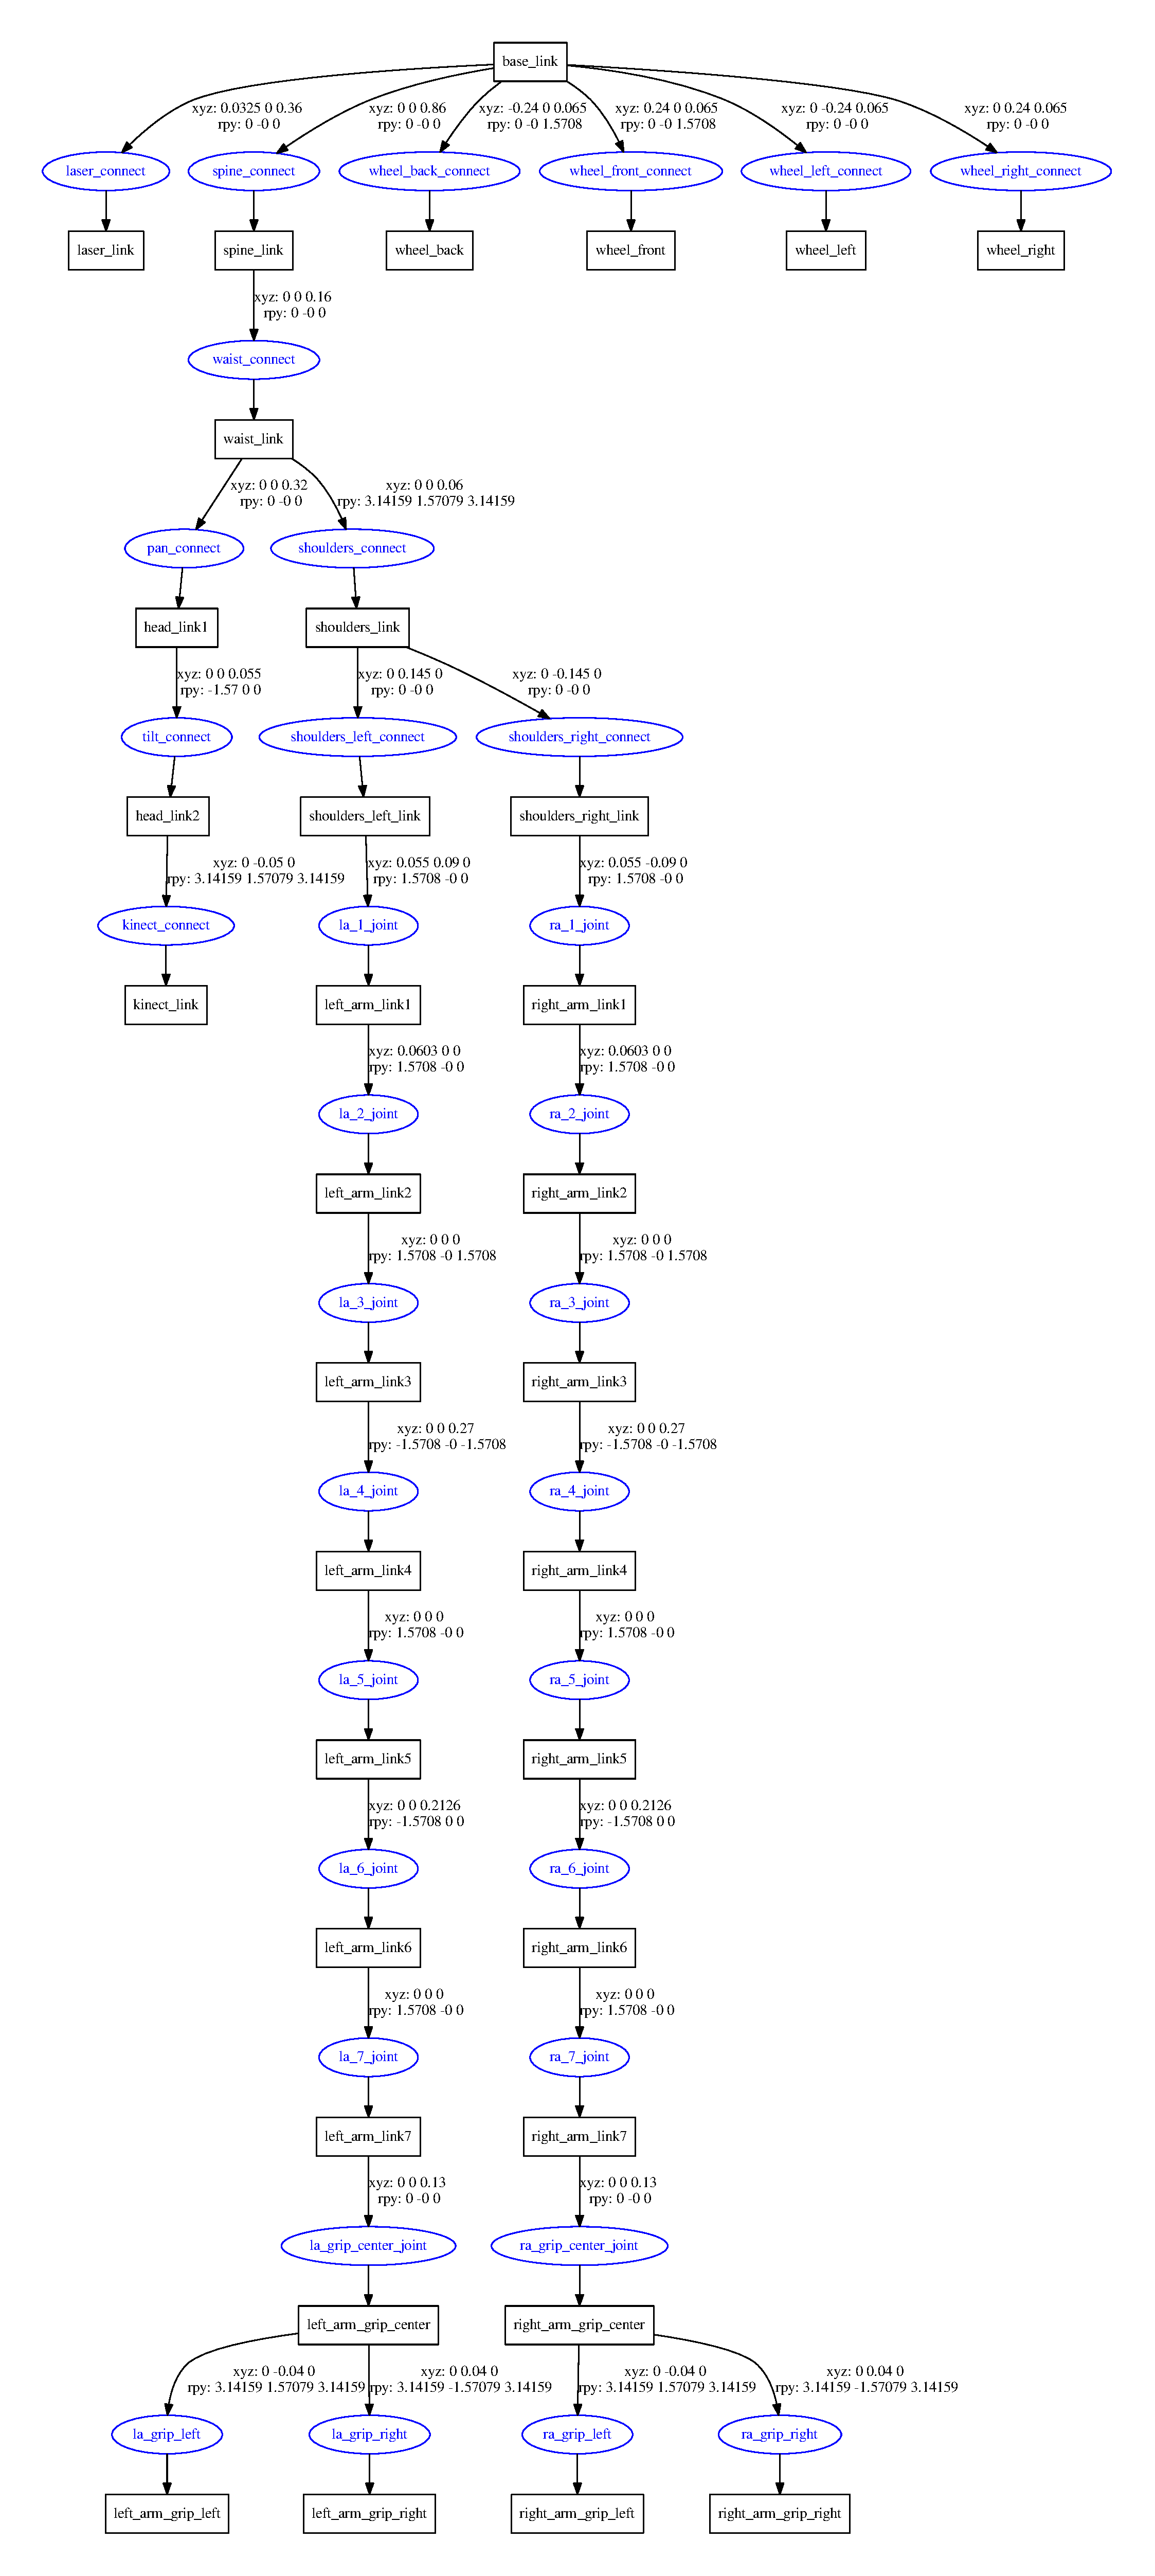
\includegraphics[scale=0.21]{Figures/Software/kinematic_tree/justina.pdf}
\end{center}
\caption{Árbol de transformaciones}
\label{fig:Sofware:Arbol}
\end{figure}

\begin{figure}[H]
\begin{center}
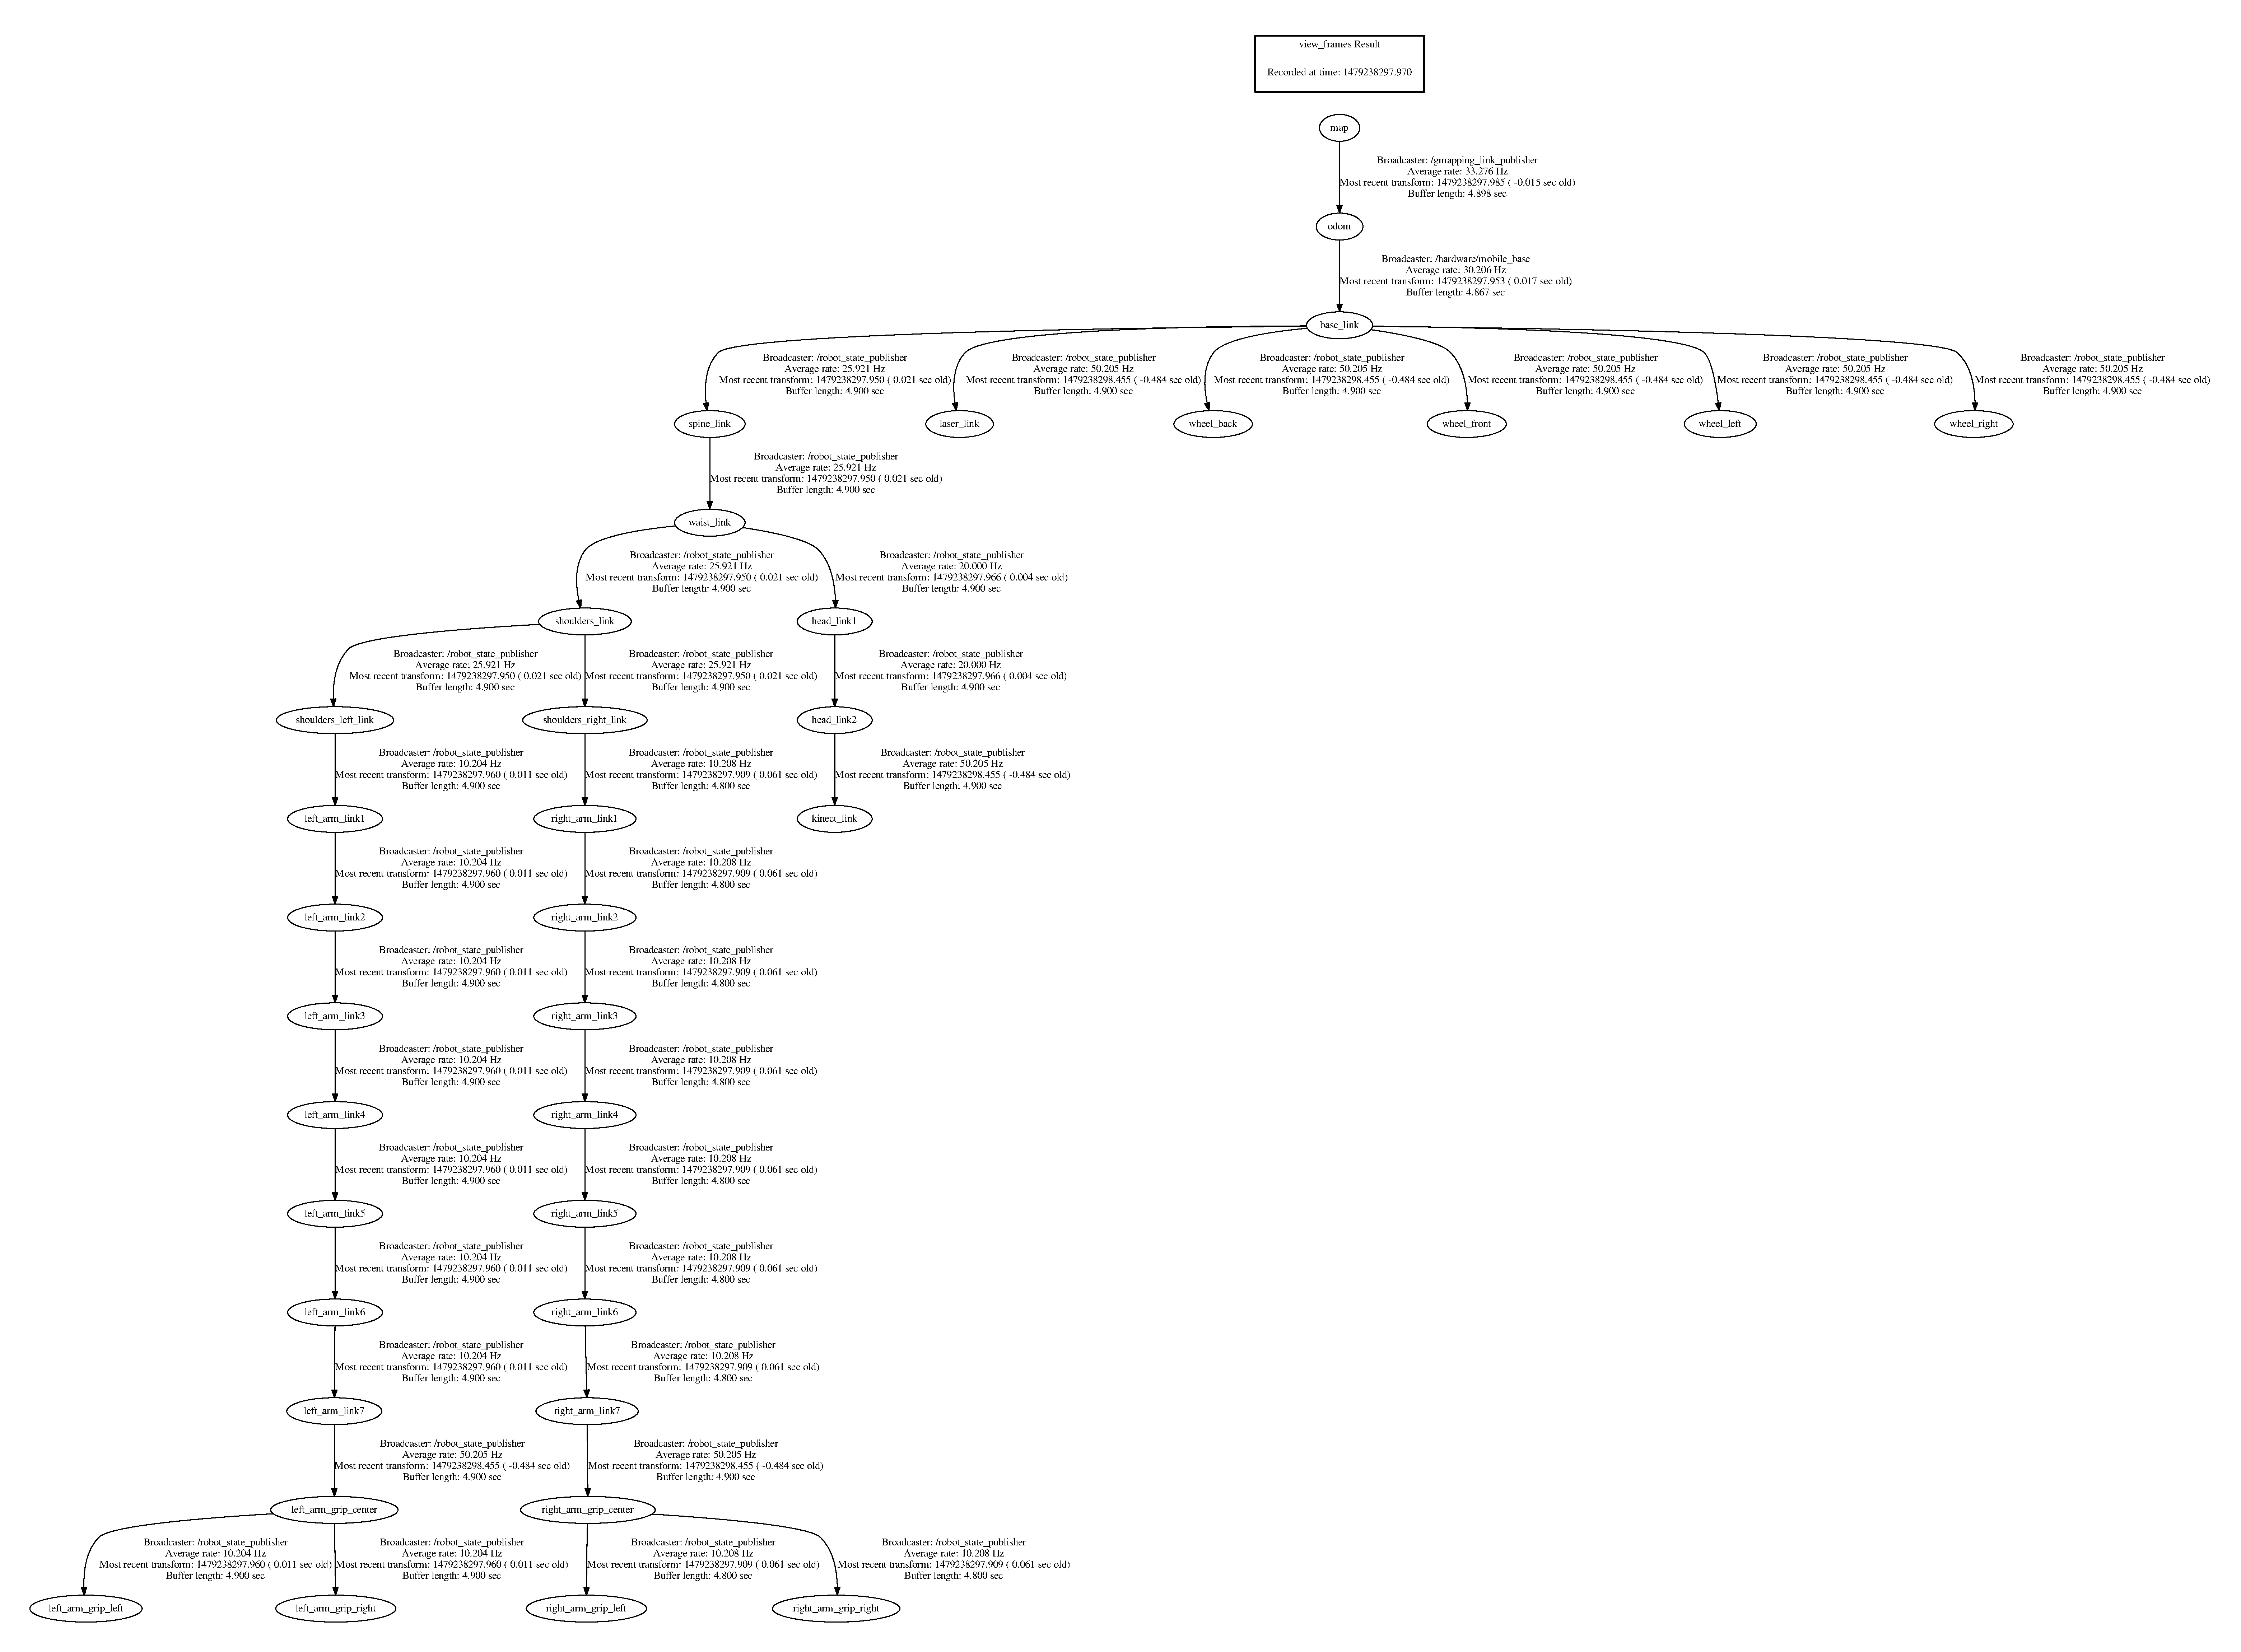
\includegraphics[scale=0.2, angle=90]{Figures/Software/kinematic_tree/frames.pdf}
\end{center}
\caption{Árbol de transformaciones con los marcos de referencia \textit{map} y \textit{odom}}
\label{fig:Sofware:Frames}
\end{figure}

%*************************************************************************************
%*************************************************************************************

\subsection{Nodo /hardware/head}
Este nodo se encarga de controlar la posición de la cabeza mediante los grados de libertad \textit{pan} y \textit{tilt}. La posición deseada se establece en radianes, en caso de que estos valores se encuentren fuera del rango de alcance de la junta, entonces  se posicionará en la cota superior o inferior según sea el caso.

%Principio de la tabla
\begin{table}[H]
\begin{center}
\begin{tabular}{|l|p{6.5cm}|p{4.5cm}|}%Define el número de columnas
\hline

Tópicos suscritos &  /hardware/head/goal\_pose [std\_msgs/Float32MultiArray] & Posición deseada de las juntas de revolución de la cabeza \\ 
& & \\
\hline

\multirow{4}{*}{Tópicos publicados} 
&  /hardware/head/current\_pose [std\_msgs/Float32MultiArray]  & Posición actual de las juntas de la cabeza \\
& & \\
%& /tf (tf/tfMessage)  & Description\\
%& & \\
& /joint\_states [sensor\_msgs/JointState] & Descripción del estado de las juntas de la cabeza \\
& & \\
& /hardware/robot\_state/head\_battery [std\_msgs/Float32]  & Voltaje de alimentación de los servo motores de la cabeza\\ 
& & \\
\cline{1-3}

\end{tabular}
\caption{Nodo /hardware/head}
\label{head node}
\end{center}
\end{table}
%Fin de la tabla

\textbf{Sintaxis en un archivo launch}\\
%Pasar argumentos y lanzar el nodo.
Para correr este nodo es necesario indicar como argumentos el puerto serial en el cual esta conectado el dispositivo \textit{USB2Dynamixel} asociado a los servo motores de la cabeza, así como el baudaje al cual se establecerá la comunicación.\\
\begin{minted}[
frame=lines,
framesep=1mm,
baselinestretch=1.2
]{xml}
<node name="head" pkg="head" type="head_node.py" output="screen" args="--port 
/dev/justinaHead --baud 1000000"/>
\end{minted}
%\fbox{\parbox[b]{\linewidth}{ \texttt{$<$node name=``head'' pkg=``head'' type=``head\_node.py'' output=``screen'' \\args=``--port /dev/justinaHead --baud 1000000''/$>$
%}}}\\

%*************************************************************************************
%*************************************************************************************

\subsection{Nodo /hardware/hokuyo\_node}
Este nodo se encarga de la adquisición de datos en un sensor Hokuyo Láser y, los hace accesibles mediante un mensaje de tipo \textit{LaserScan}. Los escaneos del Hokuyo se toman en sentido contrario a las agujas del reloj, así mismo, los ángulos se miden en sentido contrario a las agujas del reloj con 0 apuntando directamente hacia delante.
%Principio de la tabla
\begin{table}[H]
\begin{center}
\begin{tabular}{|l|p{6.5cm}|p{4.5cm}|}%Define el número de columnas
\hline

Tópicos publicados
& /hardware/scan [sensor\_msgs/LaserScan] & Datos de un escaneo \\
& & \\
\hline

\multirow{2}{*}{Parámetros} 
&  port [string, default: /dev/ttyACM0] & Puerto donde se encuentra el dispositivo Hokuyo \\
& & \\
& frame\_id [string, default: laser]  & Marco de referencia asociado al láser \\
& & \\
\cline{1-3}

\end{tabular}
\caption{Nodo /hardware/hokuyo\_node}
\label{hokuyo node}
\end{center}
\end{table}
%Fin de la tabla

\textbf{Sintaxis en un archivo launch}\\
%Pasar argumentos y lanzar el nodo.
Para lanzar este nodo por medio de un archivo \textit{lauch} es necesario indicar como parámetros el puerto en el que se encuentra el dispositivo y el marco de referencia asociado al láser, dicho marco se encuentra definido en el archivo \textit{justina.xml}.\\
\begin{minted}[
frame=lines,
framesep=1mm,
baselinestretch=1.2
]{xml}
<node name="hokuyo_node" pkg="hokuyo_node" type="hokuyo_node" output="screen">
    <param name="port" type="string" value="/dev/justinaHokuyo" />
    <param name="frame_id" type="string" value="laser_link" />
</node>
\end{minted}
%*************************************************************************************
%*************************************************************************************

\subsection{Nodo /hardware/joy}
Este nodo conecta un joystick genérico de Linux a ROS; publica un mensaje de tipo \textit{Joy} que contiene el estado actual de cada uno de los botones y ejes del joystick.

%Principio de la tabla
\begin{table}[H]
\begin{center}
\begin{tabular}{|l|p{6.5cm}|p{4.5cm}|}%Define el número de columnas
\hline

Tópicos publicados
& /hardware/joy [sensor\_msgs/Joy] & Reporta el estado de los ejes y botones del joystick \\
& & \\
\hline

Parámetros
&  dev [string, default: /dev/input/js0] & Dispositivo desde el cual se leen los eventos \\
& & \\
\hline

\end{tabular}
\caption{Nodo /hardware/joy}
\label{joy node}
\end{center}
\end{table}
%Fin de la tabla

\textbf{Sintaxis en un archivo launch}\\
Para lanzar este nodo por medio de un archivo \textit{lauch} únicamente es necesario indicar el nombre que se le desea dar al nodo, el paquete en el que se encuentra y el nombre del ejecutable.
\\
\begin{minted}[
frame=lines,
framesep=1mm,
baselinestretch=1.2
]{xml}
<node name="joy" pkg="joy" type="joy_node" output="screen"/>
\end{minted}
%*************************************************************************************
%*************************************************************************************

\subsection{Nodo /hardware/left\_arm}
Este nodo se encarga de controlar la posición de los 7 grados de libertad del brazo izquierdo del robot Justina, de igual modo controla el agarre del \textit{gripper}; la posición deseada para cada uno de los GDL se establece en radianes.
%Principio de la tabla
\begin{table}[H]
\begin{center}
\begin{tabular}{|l|p{6.5cm}|p{4.5cm}|}%Define el número de columnas
\hline

\multirow{5}{*}{Tópicos publicados}
& /hardware/left\_arm/current\_pose [std\_msgs/Float32MultiArray] & Posición actual de las juntas del brazo izquierdo \\
& & \\
& /hardware/left\_arm/current\_gripper [std\_msgs/Float32] & Posición actual del gripper \\
& & \\
%& /tf (tf/tfMessage) &  \\
%& & \\
& /joint\_states [sensor\_msgs/JointState] & Descripción del estado de las juntas del brazo izquierdo \\
& & \\
& /hardware/robot\_state/left\_arm\_battery [std\_msgs/Float32] & Voltaje de alimentación de los servo motores del brazo izquierdo \\
& & \\
\cline{1-3}

\multirow{3}{*}{Tópicos suscritos}
& /hardware/left\_arm/goal\_gripper [std\_msgs/Float32] & Posición deseada del gripper \\
& & \\
& /hardware/left\_arm/torque\_gripper [std\_msgs/Float32] & Par deseado en el gripper para tareas de manipulación de objetos \\
& & \\
& /hardware/left\_arm/goal\_pose [std\_msgs/Float32MultiArray] & Posición deseada de las juntas de revolución del brazo izquierdo. Si se especifican 7 datos, éstos serán las posiciones deseadas de los 7 GDL, si son 14 datos, los 7 adicionales serán las rapideces de los servo motores a las que se desea alcanzar dicha posición \\
& & \\
\cline{1-3}

\end{tabular}
\caption{Nodo /hardware/left\_arm}
\label{left arm node}
\end{center}
\end{table}
%Fin de la tabla

\textbf{Sintaxis en un archivo launch}\\
Para correr este nodo es necesario indicar como argumentos el puerto serial en el cual esta conectado el dispositivo \textit{USB2Dynamixel} asociado a los servo motores del brazo izquierdo, además del baudaje al cual se establecerá la comunicación.\\
\begin{minted}[
frame=lines,
framesep=1mm,
baselinestretch=1.2
]{xml}
<node name="left_arm" pkg="arms" type="left_arm_node.py" output="screen" args="--port1 
/dev/justinaLeftArm --baud1 1000000"/>
\end{minted}

%*************************************************************************************
%*************************************************************************************

\subsection{Nodo /hardware/mobile\_base}
Este nodo se encarga de controlar el movimiento de la base estableciendo la rapidez de los motores por medio de controladores \textit{RoboClaw}, la velocidad y rapidez lineal están dadas en metros por segundo y, la velocidad angular en radianes por segundo. Aparte de esto, se determina la ubicación del robot en un mapa estático utilizando \textit{tf} y un mensaje de tipo \textit{Odometry}, para obtener información más detallada consulte por favor: \url{http://wiki.ros.org/navigation/Tutorials/RobotSetup/Odom}.
%Principio de la tabla
\begin{table}[H]
\begin{center}
\begin{tabular}{|l|p{5.5cm}|p{5.5cm}|}%Define el número de columnas
\hline

\multirow{3}{*}{Tópicos publicados}
& /hardware/mobile\_base/odometry [nav\_msgs/Odometry] & Odometría calculada con las lecturas de los encoder de los motores\\
& & \\
& /hardware/robot\_state/base\_battery [std\_msgs/Float32] & Voltaje de alimentación de los motores de la base \\
& & \\
%& /tf (tf/tfMessage) &  \\
%& & \\
\cline{1-3}

\multirow{3}{*}{Tópicos suscritos}
& /hardware/robot\_state/stop [std\_msgs/Empty] & Tópico para parar los motores de la base \\
& & \\
& /hardware/mobile\_base/cmd\_vel [geometry\_msgs/Twist] & Velocidad lineal deseada en el plano \textit{xy}, y velocidad angular deseada en \textit{z} \\
& & \\
& /hardware/mobile\_base/speeds [std\_msgs/Float32MultiArray] & Rapideces instantáneas derecha e izquierda deseadas \\
& & \\
\cline{1-3}

\end{tabular}
\caption{Nodo /hardware/mobile\_base}
\label{mobile base node}
\end{center}
\end{table}
%Fin de la tabla

\textbf{Sintaxis en un archivo launch}\\
La base móvil con la que cuenta el robot Justina actualmente posee cuatro motores, es por ello que se requieren dos controladores \textit{RoboClaw}. Para lanzar este nodo se especifica mediante argumentos los dos puertos en los cuales están conectados los controladores.\\
\begin{minted}[
frame=lines,
framesep=1mm,
baselinestretch=1.2
]{xml}
<node name="mobile_base" pkg="mobile_base" type="omni_base_node.py" output="screen" 
args="--port1 /dev/justinaRC15 --port2 /dev/justinaRC30"/>
\end{minted}

%*************************************************************************************
%*************************************************************************************

\subsection{Nodo /hardware/torso}
 
%Principio de la tabla
\begin{table}[H]
\begin{center}
\begin{tabular}{|l|p{6cm}|p{5cm}|}%Define el número de columnas
\hline

\multirow{4}{*}{Tópicos publicados}
& /hardware/torso/goal\_reached [std\_msgs/Bool] &  \\
& & \\
& /tf [tf/tfMessage] &  \\
& & \\
& /joint\_states \newline[sensor\_msgs/JointState] &  \\
& & \\
& /hardware/torso/current\_pose [std\_msgs/Float32MultiArray] &  \\
& & \\
\cline{1-3}

\multirow{2}{*}{Tópicos suscritos}
& /hardware/torso/goal\_pose [std\_msgs/Float32MultiArray] &  \\
& & \\
& /hardware/torso/goal\_rel\_pose [std\_msgs/Float32MultiArray] &  \\
& & \\
\cline{1-3} 

\end{tabular}
\caption{Nodo /hardware/torso}
\label{torso node}
\end{center}
\end{table}
%Fin de la tabla

%*************************************************************************************
%*************************************************************************************

\subsection{Nodo /hri/human\_follower}
 
%Principio de la tabla
\begin{table}[H]
\begin{center}
\begin{tabular}{|l|p{6cm}|p{5cm}|}%Define el número de columnas
\hline

Tópicos publicados
& /hardware/mobile\_base/speeds [std\_msgs/Float32MultiArray] &  \\
& & \\
\hline

\multirow{2}{*}{Tópicos suscritos}
& /hri/human\_following/start\_follow [std\_msgs/Bool] &  \\
& & \\
& /hri/leg\_finder/leg\_poses \newline[geometry\_msgs/PointStamped] &  \\
& & \\
\cline{1-3}

\end{tabular}
\caption{Nodo /hri/human\_follower}
\label{human follower node}
\end{center}
\end{table}
%Fin de la tabla

%*************************************************************************************
%*************************************************************************************

\subsection{Nodo /hri/justina\_gui}
 
%Principio de la tabla
\begin{table}[H]
\begin{center}
\begin{tabular}{|l|p{6cm}|p{5cm}|}%Define el número de columnas
\hline

\multirow{4}{*}{Tópicos publicados}
& /hardware/point\_cloud\_man/save\_cloud [std\_msgs/String] &  \\
& & \\
& /navigation/path\_planning/ \newline simple\_move/goal\_lateral [std\_msgs/Float32] &  \\
& & \\
& /hardware/torso/goal\_pose [std\_msgs/Float32MultiArray] &  \\
& & \\
& /manipulation/manip\_pln/hd\_goto\_loc [std\_msgs/String] &  \\
& & \\
& /hardware/robot\_state/stop [std\_msgs/Empty] &  \\
& & \\
& /vision/face\_recognizer/start\_recog\_old [std\_msgs/Empty] &  \\
& & \\
& /manipulation/manip\_pln/ra\_goto\_loc [std\_msgs/String] &  \\
& & \\
& /manipulation/manip\_pln/ \newline la\_goto\_angles [std\_msgs/Float32MultiArray] &  \\
& & \\
& /manipulation/manip\_pln/ \newline la\_pose\_wrt\_robot [std\_msgs/Float32MultiArray] &  \\
& & \\
& /navigation/path\_planning/ \newline simple\_move/goal\_dist [std\_msgs/Float32] &  \\
& & \\

\cline{1-3}
\end{tabular}
\caption{Nodo /hri/justina\_gui}
\label{justina gui node t1}
\end{center}
\end{table}
%Fin de la tabla



%Principio de la tabla
\begin{table}[H]
\begin{center}
\begin{tabular}{|l|p{6cm}|p{5cm}|}%Define el número de columnas
\hline

\multirow{4}{*}{Tópicos publicados}
& /vision/face\_recognizer/ \newline run\_face\_recognizer\_id [std\_msgs/String] &  \\
& & \\
& /hardware/point\_cloud\_man/ \newline stop\_saving\_cloud [std\_msgs/Empty] &  \\
& & \\
& /hardware/mobile\_base/cmd\_vel \newline [geometry\_msgs/Twist] &  \\
& & \\
& /manipulation/manip\_pln/ \newline ra\_pose\_wrt\_robot [std\_msgs/Float32MultiArray] &  \\
& & \\
& /navigation/mvn\_pln/get\_close\_xya [std\_msgs/Float32MultiArray] &  \\
& & \\
& /hardware/right\_arm/goal\_torque [std\_msgs/Float32MultiArray] &  \\
& & \\
& /manipulation/manip\_pln/la\_move [std\_msgs/String] &  \\
& & \\
& /navigation/mvn\_pln/get\_close\_loc [std\_msgs/String] &  \\
& & \\
& /vision/obj\_reco/enableRecognizeTopic [std\_msgs/Bool] &  \\
& & \\
& /hardware/left\_arm/goal\_gripper [std\_msgs/Float32] &  \\
& & \\

\cline{1-3}
\end{tabular}
\caption{Nodo /hri/justina\_gui}
\label{justina gui node t2}
\end{center}
\end{table}
%Fin de la tabla



%Principio de la tabla
\begin{table}[H]
\begin{center}
\begin{tabular}{|l|p{6cm}|p{5cm}|}%Define el número de columnas
\hline

\multirow{4}{*}{Tópicos publicados}
& /hardware/mobile\_base/speeds [std\_msgs/Float32MultiArray] &  \\
& & \\
& /recognizedSpeech [hri\_msgs/RecognizedSpeech] &  \\
& & \\
& /hardware/head/goal\_pose [std\_msgs/Float32MultiArray] &  \\
& & \\
& /navigation/path\_planning/ \newline simple\_move/goal\_rel\_pose \newline [geometry\_msgs/Pose2D] &  \\
& & \\
& /hri/human\_following/start\_follow [std\_msgs/Bool] &  \\
& & \\
& /vision/obj\_reco/enableDetectWindow [std\_msgs/Bool] &  \\
& & \\
& /hardware/right\_arm/torque\_gripper [std\_msgs/Float32] &  \\
& & \\
& /vision/face\_recognizer/ \newline run\_face\_trainer\_frames \newline [vision\_msgs/VisionFaceTrainObject] &  \\
& & \\
& /hardware/torso/goal\_rel\_pose [std\_msgs/Float32MultiArray] &  \\
& & \\
& /navigation/obs\_avoid/enable [std\_msgs/Bool] &  \\
& & \\

\cline{1-3}
\end{tabular}
\caption{Nodo /hri/justina\_gui}
\label{justina gui node t3}
\end{center}
\end{table}
%Fin de la tabla





%Principio de la tabla
\begin{table}[H]
\begin{center}
\begin{tabular}{|l|p{6cm}|p{5cm}|}%Define el número de columnas
\hline

\multirow{4}{*}{Tópicos publicados}
& /vision/thermal\_vision/stop\_video [std\_msgs/Empty] &  \\
& & \\
& /vision/skeleton\_finder/stop\_recog [std\_msgs/Empty] &  \\
& & \\
& /vision/face\_recognizer/clearfacesdb [std\_msgs/Empty] &  \\
& & \\
& /manipulation/manip\_pln/ \newline hd\_goto\_angles [std\_msgs/Float32MultiArray] &  \\
& & \\
& /hardware/left\_arm/goal\_torque [std\_msgs/Float32MultiArray] &  \\
& & \\
& /vision/face\_recognizer/clearfacesdbbyid [std\_msgs/String] &  \\
& & \\
& /hardware/left\_arm/torque\_gripper [std\_msgs/Float32] &  \\
& & \\
& /navigation/path\_planning/ \newline simple\_move/goal\_dist\_angle [std\_msgs/Float32MultiArray] &  \\
& & \\
& /manipulation/manip\_pln/ \newline la\_pose\_wrt\_arm [std\_msgs/Float32MultiArray] &  \\
& & \\
& /hardware/left\_arm/goal\_pose [std\_msgs/Float32MultiArray] &  \\
& & \\

\cline{1-3}
\end{tabular}
\caption{Nodo /hri/justina\_gui}
\label{justina gui node t4}
\end{center}
\end{table}
%Fin de la tabla






%Principio de la tabla
\begin{table}[H]
\begin{center}
\begin{tabular}{|l|p{6cm}|p{5cm}|}%Define el número de columnas
\hline

\multirow{4}{*}{Tópicos publicados}
& /navigation/mvn\_pln/add\_location \newline [navig\_msgs/Location] &  \\
& & \\
& /hri/leg\_finder/enable [std\_msgs/Bool] &  \\
& & \\
& /vision/face\_recognizer/ \newline run\_face\_recognizer [std\_msgs/Empty] &  \\
& & \\
& /hri/sp\_rec/recognized [std\_msgs/String] &  \\
& & \\
& /vision/thermal\_vision/start\_video [std\_msgs/Empty] &  \\
& & \\
& /vision/face\_recognizer/run\_face\_trainer [std\_msgs/String] &  \\
& & \\
& /manipulation/manip\_pln/la\_goto\_loc [std\_msgs/String] &  \\
& & \\
& /vision/face\_recognizer/stop\_recog [std\_msgs/Empty] &  \\
& & \\
& /hardware/right\_arm/goal\_pose [std\_msgs/Float32MultiArray] &  \\
& & \\
& /vision/face\_recognizer/start\_recog [std\_msgs/Empty] &  \\
& & \\

\cline{1-3}
\end{tabular}
\caption{Nodo /hri/justina\_gui}
\label{justina gui node t5}
\end{center}
\end{table}
%Fin de la tabla




%Principio de la tabla
\begin{table}[H]
\begin{center}
\begin{tabular}{|l|p{6cm}|p{5cm}|}%Define el número de columnas
\hline

\multirow{4}{*}{Tópicos publicados}
& /navigation/path\_planning/simple\_move \newline /goal\_path [nav\_msgs/Path]  &  \\
& & \\
& /vision/skeleton\_finder/start\_recog [std\_msgs/Empty] &  \\
& & \\
& /navigation/path\_planning/simple\_move \newline /goal\_pose [geometry\_msgs/Pose2D] &  \\
& & \\
& /vision/qr/start\_qr [std\_msgs/Bool] &  \\
& & \\
& /manipulation/manip\_pln \newline /ra\_goto\_angles [std\_msgs/Float32MultiArray] &  \\
& & \\
& /hardware/right\_arm/goal\_gripper [std\_msgs/Float32] &  \\
& & \\
& /manipulation/manip\_pln \newline /ra\_pose\_wrt\_arm [std\_msgs/Float32MultiArray] &  \\
& & \\

\cline{1-3}
\end{tabular}
\caption{Nodo /hri/justina\_gui}
\label{justina gui node t6}
\end{center}
\end{table}
%Fin de la tabla






%Principio de la tabla
\begin{table}[H]
\begin{center}
\begin{tabular}{|l|p{6cm}|p{5cm}|}%Define el número de columnas
\hline

\multirow{4}{*}{Tópicos suscritos}
& /hardware/left\_arm/current\_pose [std\_msgs/Float32MultiArray] &  \\
& & \\
& /hardware/robot\_state/stop [std\_msgs/Empty] &  \\
& & \\
& /vision/face\_recognizer/faces \newline [vision\_msgs/VisionFaceObjects] &  \\
& & \\
& /recognizedSpeech [hri\_msgs/RecognizedSpeech] &  \\
& & \\
& /hardware/left\_arm/current\_gripper [std\_msgs/Float32] &  \\
& & \\
& /hri/leg\_finder/legs\_found [std\_msgs/Empty] &  \\
& & \\
& /hardware/right\_arm/current\_gripper [] &  \\
& & \\
& /navigation/localization/current\_pose [geometry\_msgs/ \newline PoseWithCovarianceStamped] &  \\
& & \\
& /hardware/head/current\_pose [std\_msgs/Float32MultiArray] &  \\
& & \\
& /hardware/torso/goal\_reached [std\_msgs/Bool] &  \\
& & \\


\cline{1-3}
\end{tabular}
\caption{Nodo /hri/justina\_gui}
\label{justina gui node t6}
\end{center}
\end{table}
%Fin de la tabla



%Principio de la tabla
\begin{table}[H]
\begin{center}
\begin{tabular}{|l|p{6cm}|p{5cm}|}%Define el número de columnas
\hline

\multirow{4}{*}{Tópicos suscritos}
& /tf [tf/tfMessage] &  \\
& & \\
& /navigation/obs\_avoid/obs\_in\_front [std\_msgs/Bool] &  \\
& & \\
& /tf\_static [tf2\_msgs/TFMessage] &  \\
& & \\
& /manipulation/hd\_goal\_reached [std\_msgs/Bool] &  \\
& & \\
& /hri/sp\_rec/recognized [std\_msgs/String] &  \\
& & \\
& /hardware/robot\_state/ \newline right\_arm\_battery [] &  \\
& & \\
& /hardware/right\_arm/current\_pose [] &  \\
& & \\
& /hardware/torso/current\_pose [std\_msgs/Float32MultiArray] &  \\
& & \\
& /manipulation/ra\_goal\_reached [std\_msgs/Bool] &  \\
& & \\
& /navigation/global\_goal\_reached [std\_msgs/Bool] &  \\
& & \\

\cline{1-3}
\end{tabular}
\caption{Nodo /hri/justina\_gui}
\label{justina gui node t7}
\end{center}
\end{table}
%Fin de la tabla





%Principio de la tabla
\begin{table}[H]
\begin{center}
\begin{tabular}{|l|p{6cm}|p{5cm}|}%Define el número de columnas
\hline

\multirow{4}{*}{Tópicos suscritos}
& /navigation/obs\_avoid/collision\_risk [std\_msgs/Bool] &  \\
& & \\
& /navigation/goal\_reached [std\_msgs/Bool] &  \\
& & \\
& /vision/face\_recognizer/trainer\_result [std\_msgs/Int32] &  \\
& & \\
& /hardware/robot\_state/left\_arm\_battery [std\_msgs/Float32] &  \\
& & \\
& /hardware/robot\_state/head\_battery [std\_msgs/Float32] &  \\
& & \\
& /hri/qr/recognized [std\_msgs/String] &  \\
& & \\
& /manipulation/la\_goal\_reached [std\_msgs/Bool] &  \\
& & \\
& /hardware/robot\_state/base\_battery [std\_msgs/Float32] &  \\
& & \\ 

\cline{1-3}
\end{tabular}
\caption{Nodo /hri/justina\_gui}
\label{justina gui node t7}
\end{center}
\end{table}
%Fin de la tabla

%*************************************************************************************
%*************************************************************************************

\subsection{Nodo /hri/leg\_finder}
 
%Principio de la tabla
\begin{table}[H]
\begin{center}
\begin{tabular}{|l|p{6cm}|p{5cm}|}%Define el número de columnas
\hline

\multirow{2}{*}{Tópicos publicados}
& /hri/leg\_finder/legs\_found [std\_msgs/Empty] &  \\
& & \\
& /hri/leg\_finder/leg\_poses \newline [geometry\_msgs/PointStamped] &  \\
& & \\
\cline{1-3}

\multirow{4}{*}{Tópicos suscritos}
& /hardware/scan \newline [sensor\_msgs/LaserScan] &  \\
& & \\
& /tf [tf/tfMessage] &  \\
& & \\
& /tf\_static [tf2\_msgs/TFMessage] &  \\
& & \\
& /hri/leg\_finder/enable [std\_msgs/Bool]  &  \\
& & \\
\cline{1-3}

\end{tabular}
\caption{Nodo /hri/leg\_finder}
\label{leg finder node}
\end{center}
\end{table}
%Fin de la tabla

%*************************************************************************************
%*************************************************************************************

\subsection{Nodo /hri/qr\_reader}
 
%Principio de la tabla
\begin{table}[H]
\begin{center}
\begin{tabular}{|l|p{6cm}|p{5cm}|}%Define el número de columnas
\hline

Tópicos publicados
& /hri/qr/recognized [std\_msgs/String] &  \\
& & \\
\hline

\multirow{3}{*}{Tópicos suscritos}
& /tf [tf/tfMessage] &  \\
& & \\
& /tf\_static [tf2\_msgs/TFMessage] &  \\
& & \\
& /vision/qr/start\_qr [std\_msgs/Bool] &  \\
& & \\
\cline{1-3}

\end{tabular}
\caption{Nodo /hri/qr\_reader}
\label{qr reader node}
\end{center}
\end{table}
%Fin de la tabla

%*************************************************************************************
%*************************************************************************************

\subsection{Nodo /hri/rviz}
 
%Principio de la tabla
\begin{table}[H]
\begin{center}
\begin{tabular}{|l|p{6cm}|p{5cm}|}%Define el número de columnas
\hline

\multirow{3}{*}{Tópicos publicados}
& /clicked\_point \newline [geometry\_msgs/PointStamped] &  \\
& & \\
& /move\_base\_simple/goal \newline [geometry\_msgs/PoseStamped] &  \\
& & \\
& /initialpose \newline [geometry\_msgs/ \newline PoseWithCovarianceStamped] &  \\
& & \\
\cline{1-3}

\multirow{9}{*}{Tópicos suscritos}
& /hri/rviz/location\_markers \newline [visualization\_msgs/Marker] &  \\
& & \\
& /hardware/scan \newline [sensor\_msgs/LaserScan]  &  \\
& & \\
& /hri/rviz/location\_markers\_array \newline [] &  \\
& & \\
& /tf [tf/tfMessage] &  \\
& & \\
& /tf\_static [tf2\_msgs/TFMessage] &  \\
& & \\
& /hri/leg\_finder/leg\_poses \newline [geometry\_msgs/PointStamped] &  \\
& & \\
& /navigation/localization/map\_updates [] &  \\
& & \\
& /navigation/mvn\_pln/last\_calc\_path [nav\_msgs/Path] &  \\
& & \\
& /navigation/localization/map [nav\_msgs/OccupancyGrid] &  \\
& & \\
\cline{1-3}

\end{tabular}
\caption{Nodo /hri/rviz}
\label{rviz node}
\end{center}
\end{table}
%Fin de la tabla

%*************************************************************************************
%*************************************************************************************

\subsection{Nodo /hri/sp\_gen}
 
%Principio de la tabla
\begin{table}[H]
\begin{center}
\begin{tabular}{|l|p{6cm}|p{5cm}|}%Define el número de columnas
\hline

Tópicos suscritos
& /hri/sp\_gen/say [] &  \\
& & \\
\hline

\end{tabular}
\caption{Nodo /hri/sp\_gen}
\label{sp gen node}
\end{center}
\end{table}
%Fin de la tabla

%*************************************************************************************
%*************************************************************************************

\subsection{Nodo /interoperation/joystick\_teleop}
Este nodo se suscribe a un mensaje de tipo \textit{Joy} para controlar mediante un joystick de una consola Xbox el movimiento de la base, la posición de la cabeza y del torso. Las posiciones angulares y lineales, así como las velocidades lineales y angulares están dadas en radianes, metros, metros por segundo y radianes por segundo respectivamente.\\

Para mover la cabeza del robot se utiliza el \textit{stick} izquierdo, la base se opera por medio del \textit{stick} derecho, mientras que el botón rojo del joystick es para el paro de la base.\\

%Principio de la tabla
\begin{table}[H]
\begin{center}
\begin{tabular}{|l|p{6cm}|p{5cm}|}%Define el número de columnas
\hline

\multirow{6}{*}{Tópicos publicados}
& /hardware/robot\_state/stop [std\_msgs/Empty] & Tópico de paro para los motores de la base \\
& & \\
& /hardware/mobile\_base/cmd\_vel \newline [geometry\_msgs/Twist] & Velocidad lineal deseada deseada de la base en el plano \textit{xy}, y velocidad angular deseada en \textit{z} \\
& & \\
& /hardware/head/goal\_pose [std\_msgs/Float32MultiArray] & Posición deseada de la cabeza \\
& & \\
& /hardware/torso/goal\_spine [std\_msgs/Float32] & Posición deseada de la junta prismática para cambiar la altura del torso \\
& & \\
& /hardware/torso/goal\_shoulders [std\_msgs/Float32] & Posición deseada de la junta de revolución para orientar el torso (roll) \\
& & \\
& /hardware/torso/goal\_waist [std\_msgs/Float32] & Posición deseada de la junta de revolución para orientar el torso (yaw) \\
& & \\
\cline{1-3}

Tópicos suscritos
& /hardware/joy [sensor\_msgs/Joy]  & Estado de los ejes y botones de un joystick \\
& & \\
\hline

\end{tabular}
\caption{Nodo /interoperation/joystick\_teleop}
\label{joystick teleop node}
\end{center}
\end{table}
%Fin de la tabla

\textbf{Sintaxis en un archivo launch}\\
Para lanzar este nodo por medio de un archivo \textit{lauch} sólo se necesita indicar el nombre que se le desea dar al nodo, el paquete dentro del que se encuentra y el nombre del ejecutable.\\
\begin{minted}[
frame=lines,
framesep=1mm,
baselinestretch=1.2
]{xml}
<node name="joystick_teleop" pkg="joystick_teleop" type="joystick_teleop_node.py" 
output="screen" />
\end{minted}

%*************************************************************************************
%*************************************************************************************
\subsection{Nodo /manipulation/ik\_geometric}
 
%Principio de la tabla
\begin{table}[H]
\begin{center}
\begin{tabular}{|l|p{6cm}|p{5cm}|}%Define el número de columnas
\hline

\multirow{4}{*}{Servicios}
& /manipulation/ik\_geometric/ \newline ik\_float\_array &  \\
& & \\
& /manipulation/ik\_geometric/ik\_path &  \\
& & \\
& /manipulation/ik\_geometric/ik\_pose &  \\
& & \\
& /manipulation/ik\_geometric/ \newline direct\_kinematics &  \\
& & \\
\cline{1-3}

\end{tabular}
\caption{Nodo /manipulation/ik\_geometric}
\label{ik geometric node}
\end{center}
\end{table}
%Fin de la tabla

%*************************************************************************************
%*************************************************************************************
\subsection{Nodo  /manipulation/manip\_pln}
 
%Principio de la tabla
\begin{table}[H]
\begin{center}
\begin{tabular}{|l|p{6cm}|p{5cm}|}%Define el número de columnas
\hline

\multirow{9}{*}{Tópicos publicados}
& /hardware/right\_arm/goal\_torque [std\_msgs/Float32MultiArray] &  \\
& & \\
& /hardware/head/goal\_pose [std\_msgs/Float32MultiArray] &  \\
& & \\
& /hardware/left\_arm/goal\_torque [std\_msgs/Float32MultiArray] &  \\
& & \\
& /hardware/left\_arm/goal\_pose [std\_msgs/Float32MultiArray] &  \\
& & \\
& /manipulation/hd\_goal\_reached [std\_msgs/Bool] &  \\
& & \\
& /manipulation/ra\_goal\_reached [std\_msgs/Bool] &  \\
& & \\
& /hardware/right\_arm/goal\_pose [std\_msgs/Float32MultiArray] &  \\
& & \\
& /hardware/head/goal\_torque [std\_msgs/Float32MultiArray]  &  \\
& & \\
& /manipulation/la\_goal\_reached [std\_msgs/Bool] &  \\
& & \\
\cline{1-3}

\end{tabular}
\caption{Nodo  /manipulation/manip\_pln }
\label{manip pln node t1}
\end{center}
\end{table}
%Fin de la tabla


%Principio de la tabla
\begin{table}[H]
\begin{center}
\begin{tabular}{|l|p{6cm}|p{5cm}|}%Define el número de columnas
\hline

\multirow{10}{*}{Tópicos suscritos}
& /hardware/left\_arm/current\_pose [std\_msgs/Float32MultiArray] &  \\
& & \\
& /manipulation/manip\_pln/ra\_goto\_loc [std\_msgs/String] &  \\
& & \\
& /manipulation/manip\_pln/hd\_goto\_loc [std\_msgs/String] &  \\
& & \\
& /manipulation/manip\_pln/ \newline la\_goto\_angles [std\_msgs/Float32MultiArray] &  \\
& & \\
& /manipulation/manip\_pln/ \newline la\_pose\_wrt\_robot [std\_msgs/Float32MultiArray] &  \\
& & \\
& /manipulation/manip\_pln/ \newline ra\_pose\_wrt\_robot [std\_msgs/Float32MultiArray] &  \\
& & \\
& /manipulation/manip\_pln/la\_move [std\_msgs/String] &  \\
& & \\
& /hardware/head/current\_pose [std\_msgs/Float32MultiArray] &  \\
& & \\
& /manipulation/manip\_pln/hd\_move [] &  \\
& & \\
& /manipulation/manip\_pln/ra\_move [] &  \\
& & \\
\cline{1-3}

\end{tabular}
\caption{Nodo  /manipulation/manip\_pln }
\label{manip pln node t2}
\end{center}
\end{table}
%Fin de la tabla


%Principio de la tabla
\begin{table}[H]
\begin{center}
\begin{tabular}{|l|p{6cm}|p{5cm}|}%Define el número de columnas
\hline

\multirow{8}{*}{Tópicos suscritos}
& /manipulation/manip\_pln/ \newline hd\_goto\_angles [std\_msgs/Float32MultiArray] &  \\
& & \\
& /tf [tf/tfMessage] &  \\
& & \\
& /manipulation/manip\_pln/ \newline la\_pose\_wrt\_arm [std\_msgs/Float32MultiArray] &  \\
& & \\
& /tf\_static [tf2\_msgs/TFMessage] &  \\
& & \\
& /hardware/right\_arm/current\_pose [] &  \\
& & \\
& /manipulation/manip\_pln/la\_goto\_loc [std\_msgs/String] &  \\
& & \\
& /manipulation/manip\_pln/ \newline ra\_pose\_wrt\_arm [std\_msgs/Float32MultiArray] &  \\
& & \\
& /manipulation/manip\_pln/ \newline ra\_goto\_angles [std\_msgs/Float32MultiArray] &  \\
& & \\
\cline{1-3}

\end{tabular}
\caption{Nodo  /manipulation/manip\_pln }
\label{manip pln node t3}
\end{center}
\end{table}
%Fin de la tabla

%*************************************************************************************
%*************************************************************************************
\subsection{Nodo /navigation/localization/loc\_amcl}
Este nodo implementa el enfoque adaptativo de localización de Monte Carlo, que utiliza un filtro de partículas para rastrear la pose de un robot en un mapa conocido. AMCL es un sistema de localización probabilística para un robot que se mueve en un plano.\\

AMCL transforma los escaneos láser entrantes al sistema de referencia \textit{odometry}. Por lo tanto, debe existir un camino a través del árbol \textit{tf} desde el sistema de referencia en el que los escaneos láser se publican hacia el sistema de referencia de odometría.\\

Durante la operación AMCL estima la transformación del marco de referencia de la base con respecto al marco de referencia global(\textit{map} para este caso), pero solamente publica la transformación entre el marco de referencia global(\textit{map}) y el marco de referencia de odometría(\textit{odometry}). Esencialmente, esta transformación considera la deriva que ocurre usando \textit{Dead Reckoning}. \textit{Dead Reckoning} es el proceso de calcular la posición estimando la dirección y la distancia recorrida.\\

Para obtener información más detallada consulte: \url{http://wiki.ros.org/amcl}.

%Principio de la tabla
\begin{table}[H]
\begin{center}
\begin{tabular}{|l|p{6cm}|p{5cm}|}%Define el número de columnas
\hline

\multirow{2}{*}{Tópicos publicados}
& /navigation/localization/current\_pose [geometry\_msgs/ \newline PoseWithCovarianceStamped] & Posición estimada del robot en el mapa, con covarianza \\
& & \\
& /tf [tf/tfMessage] & Publica la transformación de odom (que se puede reasignar a través del parámetro \textit{odom\_frame\_id}) a map \\
& & \\
& /navigation/localization/particlecloud [geometry\_msgs/PoseArray] & Conjunto de poses estimadas mantenidas por el filtro \\
& & \\
\cline{1-3}

\multirow{4}{*}{Servicios}
%& /navigation/localization/ \newline request\_nomotion\_update &  \\
%& & \\
%& /navigation/localization/set\_map &  \\
%& & \\
& /navigation/localization/ \newline global\_localization [std\_srvs/Empty] & Inicio de la localización global, donde todas las partículas se dispersan al azar a través del espacio libre en el mapa \\
& & \\
%& /navigation/localization/loc\_amcl/ \newline set\_parameters &  \\
%& & \\
\cline{1-3}

\end{tabular}
\caption{Nodo /navigation/localization/loc\_amcl}
\label{loc amcl node t1}
\end{center}
\end{table}
%Fin de la tabla

%Principio de la tabla
\begin{table}[H]
\begin{center}
\begin{tabular}{|l|p{6cm}|p{5cm}|}%Define el número de columnas
\hline

\multirow{4}{*}{Tópicos suscritos}
& /navigation/localization/initialpose \newline [geometry\_msgs/ \newline PoseWithCovarianceStamped] & Media y covarianza con la cual se (re-)inicializa el filtro de partículas \\
& & \\
& /hardware/scan \newline [sensor\_msgs/LaserScan] & Escaneos láser \\
& & \\
& /tf [tf/tfMessage] & Transformaciones del robot \\
& & \\
%& /tf\_static [tf2\_msgs/TFMessage]  &  \\
%& & \\
\cline{1-3}

\multirow{3}{*}{Parámetros}
& update\_min\_a \newline [double, default: $ \pi $/6.0 radians] & Movimiento de rotación requerido antes de realizar una actualización del filtro \\
& & \\
& laser\_min\_range [double, default: -1.0] & Rango de escaneo mínimo a considerar \\
% -1.0 hará que el rango mínimo reportado del láser sea usado \\
& & \\
& odom\_model\_type \newline [string, default: ``diff''] & Configuración del robot, ya sea ``diff'', ``omni'', ``diff-corrected'' o ``omni-corrected'' \\
& & \\
\cline{1-3}

\end{tabular}
\caption{Nodo /navigation/localization/loc\_amcl}
\label{loc amcl node t2}
\end{center}
\end{table}
%Fin de la tabla

\textbf{Sintaxis en un archivo launch}\\
Para correr este nodo se necesita indicar el tópico en el cual se publican los datos del láser (\textit{/hardware/scan} para este caso), de igual forma se requiere modificar los parámetros \textit{update\_min\_a}, \textit{laser\_min\_range} y \textit{odom\_model\_typ}.\\
\begin{minted}[
frame=lines,
framesep=1mm,
baselinestretch=1.2
]{xml}
<node name="loc_amcl" pkg="amcl" type="amcl" output="acreen" args="scan:=/hardware/scan">
    <param name="update_min_a" value="0.3"/>
    <param name="laser_min_range" value="0.3"/>
    <param name="odom_model_type" value="omni"/>
</node>
\end{minted}
%*************************************************************************************
%*************************************************************************************
\subsection{Nodo /navigation/localization/map\_server}
Este nodo ofrece datos de un mapa como un servicio de ROS. También proporciona la utilidad de línea de comandos \textit{map\_saver}, que permite guardar en un archivo los mapas generados dinámicamente.\\

Los mapas manipulados por las herramientas de este paquete se almacenan en un par de archivos, un archivo YAML describe los metadatos del mapa y una imagen codifica los datos de ocupación. La imagen describe el estado de ocupación de cada celda del mundo en el color del píxel correspondiente. Los píxeles más blancos están libres, los píxeles más negros están ocupados y los píxeles entre estos colores son desconocidos. Los campos requeridos en el archivo YAML son seis: \textit{image}, \textit{resolution}, \textit{origin}, \textit{occupied\_thresh}, \textit{free\_thresh} y \textit{negate}. \\

Para obtener información más específica por favor consulte: \url{http://wiki.ros.org/map_server}.\\

%Principio de la tabla
\begin{table}[H]
\begin{center}
\begin{tabular}{|l|p{6cm}|p{5cm}|}%Define el número de columnas
\hline

\multirow{2}{*}{Tópicos publicados}
& /navigation/localization/map\_metadata [nav\_msgs/MapMetaData] & Metadatos del mapa \\
& & \\
& /navigation/localization/map [nav\_msgs/OccupancyGrid] & Mapa  \\
& & \\
\cline{1-3}
 
Servicios
& navigation/localization/static\_map [nav\_msgs/GetMap] & Obtención del mapa a través de este servicio \\
& & \\
\hline

Parámetros
& frame\_id [string, default: ``map''] & Marco de referencia establecido en el encabezado (\textit{header}) del mapa publicado \\
& & \\
\hline

\end{tabular}
\caption{Nodo /navigation/localization/map\_server}
\label{map server node}
\end{center}
\end{table}
%Fin de la tabla

\textbf{Sintaxis en un archivo launch}\\
Para ejecutar este nodo se requiere especificar como argumento el archivo YAML que contiene los metadatos del mapa que se quiere proveer. Para este ejemplo, el archivo \textit{bioroboanexo3.yaml} se encuentra dentro del paquete \textit{knowledge} en la ruta \textit{navigation/occupancy\_grids}.\\
\begin{minted}[
frame=lines,
framesep=1mm,
baselinestretch=1.2
]{xml}
<node name="map_server" pkg="map_server" type="map_server" output="screen" 
      args="$(find knowledge)/navigation/occupancy_grids/bioroboanexo3.yaml"/>$
\end{minted}
%*************************************************************************************
%*************************************************************************************
\subsection{Nodo /navigation/mvn\_pln}
 
%Principio de la tabla
\begin{table}[H]
\begin{center}
\begin{tabular}{|l|p{6cm}|p{5cm}|}%Define el número de columnas
\hline

\multirow{9}{*}{Tópicos publicados}
& /navigation/path\_planning/simple\_move \newline /goal\_lateral [std\_msgs/Float32] &  \\
& & \\
& /hardware/torso/goal\_pose [std\_msgs/Float32MultiArray] &  \\
& & \\
& /manipulation/manip\_pln/hd\_goto\_loc [std\_msgs/String] &  \\
& & \\
& /manipulation/manip\_pln/ra\_goto\_loc [std\_msgs/String] &  \\
& & \\
& /hri/rviz/location\_markers \newline [visualization\_msgs/Marker] &  \\
& & \\
& /manipulation/manip\_pln/ \newline la\_goto\_angles [std\_msgs/Float32MultiArray] &  \\
& & \\
& /manipulation/manip\_pln/ \newline la\_pose\_wrt\_robot [std\_msgs/Float32MultiArray] &  \\
& & \\
& /navigation/path\_planning/simple\_move \newline /goal\_dist [std\_msgs/Float32] &  \\
& & \\
& /manipulation/manip\_pln/ \newline ra\_pose\_wrt\_robot [std\_msgs/Float32MultiArray] &  \\
& & \\
\cline{1-3}

\end{tabular}
\caption{Nodo /navigation/mvn\_pln}
\label{mvn pln node t1}
\end{center}
\end{table}
%Fin de la tabla

%Principio de la tabla
\begin{table}[H]
\begin{center}
\begin{tabular}{|l|p{6cm}|p{5cm}|}%Define el número de columnas
\hline

\multirow{9}{*}{Tópicos publicados}
& /navigation/mvn\_pln/get\_close\_xya [std\_msgs/Float32MultiArray] &  \\
& & \\
& /manipulation/manip\_pln/la\_move [std\_msgs/String] &  \\
& & \\
& /navigation/mvn\_pln/get\_close\_loc [std\_msgs/String] &  \\
& & \\
& /hardware/left\_arm/goal\_gripper [std\_msgs/Float32] &  \\
& & \\
& /navigation/path\_planning/simple\_move \newline /goal\_rel\_pose \newline [geometry\_msgs/Pose2D] &  \\
& & \\
& /hardware/right\_arm/torque\_gripper [std\_msgs/Float32] &  \\
& & \\
& /hardware/torso/goal\_rel\_pose [std\_msgs/Float32MultiArray] &  \\
& & \\
& /navigation/obs\_avoid/enable [std\_msgs/Bool] &  \\
& & \\
& /manipulation/manip\_pln/ \newline hd\_goto\_angles [std\_msgs/Float32MultiArray] &  \\
& & \\
\cline{1-3}

\end{tabular}
\caption{Nodo /navigation/mvn\_pln}
\label{mvn pln node t2}
\end{center}
\end{table}
%Fin de la tabla



%Principio de la tabla
\begin{table}[H]
\begin{center}
\begin{tabular}{|l|p{6cm}|p{5cm}|}%Define el número de columnas
\hline

\multirow{9}{*}{Tópicos publicados}
& /hardware/left\_arm/torque\_gripper [std\_msgs/Float32] &  \\
& & \\
& /navigation/path\_planning/simple\_move \newline /goal\_dist\_angle [std\_msgs/Float32MultiArray] &  \\
& & \\
& /manipulation/manip\_pln/ \newline la\_pose\_wrt\_arm [std\_msgs/Float32MultiArray] &  \\
& & \\
& /navigation/mvn\_pln/add\_location \newline [navig\_msgs/Location] &  \\
& & \\
& /navigation/mvn\_pln/last\_calc\_path [nav\_msgs/Path] &  \\
& & \\
& /navigation/global\_goal\_reached [std\_msgs/Bool] &  \\
& & \\
& /manipulation/manip\_pln/la\_goto\_loc [std\_msgs/String] &  \\
& & \\
& /navigation/path\_planning/simple\_move \newline /goal\_path [nav\_msgs/Path] &  \\
& & \\
& /navigation/path\_planning/simple\_move \newline /goal\_pose [geometry\_msgs/Pose2D] &  \\
& & \\
\cline{1-3}
  
\end{tabular}
\caption{Nodo /navigation/mvn\_pln}
\label{mvn pln node t3}
\end{center}
\end{table}
%Fin de la tabla

%Principio de la tabla
\begin{table}[H]
\begin{center}
\begin{tabular}{|l|p{6cm}|p{5cm}|}%Define el número de columnas
\hline

\multirow{3}{*}{Tópicos publicados}
& /manipulation/manip\_pln/ \newline ra\_goto\_angles [std\_msgs/Float32MultiArray] &  \\
& & \\
& /hardware/right\_arm/goal\_gripper [std\_msgs/Float32] &  \\
& & \\
& /manipulation/manip\_pln/ \newline ra\_pose\_wrt\_arm [std\_msgs/Float32MultiArray] &  \\
& & \\
\cline{1-3}

Servicios
& /navigation/mvn\_pln/plan\_path  &  \\
& & \\
\hline

\end{tabular}
\caption{Nodo /navigation/mvn\_pln}
\label{mvn pln node t4}
\end{center}
\end{table}
%Fin de la tabla

%Principio de la tabla
\begin{table}[H]
\begin{center}
\begin{tabular}{|l|p{6cm}|p{5cm}|}%Define el número de columnas
\hline

\multirow{9}{*}{Tópicos suscritos}
& /hardware/robot\_state/stop [std\_msgs/Empty] &  \\
& & \\
& /navigation/mvn\_pln/get\_close\_xya [std\_msgs/Float32MultiArray] &  \\
& & \\
& /clicked\_point \newline [geometry\_msgs/PointStamped] &  \\
& & \\
& /navigation/mvn\_pln/get\_close\_loc [std\_msgs/String] &  \\
& & \\
& /navigation/localization/current\_pose [geometry\_msgs/ \newline PoseWithCovarianceStamped] &  \\
& & \\
& /hardware/scan \newline [sensor\_msgs/LaserScan] &  \\
& & \\
& /hardware/torso/goal\_reached [std\_msgs/Bool] &  \\
& & \\
& /tf [tf/tfMessage]  &  \\
& & \\
& /navigation/obs\_avoid/obs\_in\_front [std\_msgs/Bool] &  \\
& & \\
\cline{1-3}

\end{tabular}
\caption{Nodo /navigation/mvn\_pln}
\label{mvn pln node t5}
\end{center}
\end{table}
%Fin de la tabla

%Principio de la tabla
\begin{table}[H]
\begin{center}
\begin{tabular}{|l|p{6cm}|p{5cm}|}%Define el número de columnas
\hline

\multirow{9}{*}{Tópicos suscritos}
& /tf\_static [tf2\_msgs/TFMessage]  &  \\
& & \\
& /manipulation/hd\_goal\_reached [std\_msgs/Bool] &  \\
& & \\
& /navigation/mvn\_pln/add\_location \newline [navig\_msgs/Location] &  \\
& & \\
& /manipulation/ra\_goal\_reached [std\_msgs/Bool] &  \\
& & \\
& /navigation/global\_goal\_reached [std\_msgs/Bool] &  \\
& & \\
& /navigation/obs\_avoid/collision\_risk [std\_msgs/Bool]  &  \\
& & \\
& /navigation/goal\_reached [std\_msgs/Bool] &  \\
& & \\
& /navigation/obs\_avoid/collision\_point [geometry\_msgs/PointStamped] &  \\
& & \\
& /manipulation/la\_goal\_reached [std\_msgs/Bool] &  \\
& & \\
\cline{1-3}

\end{tabular}
\caption{Nodo /navigation/mvn\_pln}
\label{mvn pln node t6}
\end{center}
\end{table}
%Fin de la tabla

%*************************************************************************************
%*************************************************************************************

\subsection{Nodo /navigation/obs\_avoid/obstacle\_detector}
 
%Principio de la tabla
\begin{table}[H]
\begin{center}
\begin{tabular}{|l|p{6cm}|p{5cm}|}%Define el número de columnas
\hline

\multirow{3}{*}{Tópicos publicados}
& /navigation/obs\_avoid/obs\_in\_front [std\_msgs/Bool] &  \\
& & \\
& /navigation/obs\_avoid/collision\_risk [std\_msgs/Bool] &  \\
& & \\
& /navigation/obs\_avoid/collision\_point [geometry\_msgs/PointStamped]  &  \\
& & \\
\cline{1-3}

\multirow{5}{*}{Tópicos suscritos}
& /hardware/scan \newline [sensor\_msgs/LaserScan] &  \\
& & \\
& /navigation/obs\_avoid/enable [std\_msgs/Bool]  &  \\
& & \\
& /tf [tf/tfMessage]  &  \\
& & \\
& /tf\_static [tf2\_msgs/TFMessage] &  \\
& & \\
& /navigation/mvn\_pln/last\_calc\_path [nav\_msgs/Path] &  \\
& & \\
\cline{1-3}
  
\end{tabular}
\caption{Nodo /navigation/obs\_avoid/obstacle\_detector}
\label{obs avoid obstacle detector node}
\end{center}
\end{table}
%Fin de la tabla

%*************************************************************************************
%*************************************************************************************

\subsection{Nodo /navigation/path\_planning/path\_calculator}
Este nodo se encarga de calcular una ruta y suavizarla desde una pose inicial hasta una pose objetivo utilizando el algoritmo de búsqueda A$ ^{*} $, ésto mediante dos servicios de ROS.\\
%Principio de la tabla
\begin{table}[H]
\begin{center}
\begin{tabular}{|l|p{6cm}|p{5cm}|}%Define el número de columnas
\hline

\multirow{2}{*}{Servicios}
& /navigation/path\_planning/ \newline path\_calculator/wave\_front\_from\_map [navig\_msgs/PathFromMap] &  \\
& & \\
& /navigation/path\_planning/ \newline path\_calculator/a\_star\_from\_map [navig\_msgs/PathFromMap] & Cálculo de una ruta utilizando el algoritmo de búsqueda A$ ^{*} $ \\
& & \\
\cline{1-3}

\end{tabular}
\caption{Nodo /navigation/path\_planning/path\_calculator}
\label{path calculator node}
\end{center}
\end{table}
%Fin de la tabla

\textbf{Sintaxis en un archivo launch}\\
Para correr este nodo sólo se requiere especificar el nombre que se le desea dar al nodo, el paquete en el que se encuentra y el nombre del ejecutable.\\
\begin{minted}[
frame=lines,
framesep=1mm,
baselinestretch=1.2
]{xml}
<node name="path_calculator" pkg="path_calculator" type="path_calculator_node" 
output="screen"/>
\end{minted}
%*************************************************************************************
%*************************************************************************************

\subsection{Nodo /navigation/path\_planning/simple\_move}

%Principio de la tabla
\begin{table}[H]
\begin{center}
\begin{tabular}{|l|p{6cm}|p{5cm}|}%Define el número de columnas
\hline

\multirow{4}{*}{Tópicos publicados}
& /hardware/mobile\_base/cmd\_vel \newline [geometry\_msgs/Twist] &  \\
& & \\
& /hardware/mobile\_base/speeds [std\_msgs/Float32MultiArray] &  \\
& & \\
& /hardware/head/goal\_pose [std\_msgs/Float32MultiArray] &  \\
& & \\
& /navigation/goal\_reached [std\_msgs/Bool] &  \\
& & \\
\cline{1-3}

\multirow{4}{*}{Tópicos suscritos}
& /hardware/robot\_state/stop [std\_msgs/Empty] &  \\
& & \\
& /navigation/path\_planning/simple\_move \newline /goal\_lateral [std\_msgs/Float32] &  \\
& & \\
& /navigation/path\_planning/simple\_move \newline /goal\_dist [std\_msgs/Float32] &  \\
& & \\
& /navigation/path\_planning/simple\_move \newline /goal\_rel\_pose \newline [geometry\_msgs/Pose2D] &  \\
& & \\
\cline{1-3}

\end{tabular}
\caption{Nodo /navigation/path\_planning/simple\_move}
\label{simple move node t1}
\end{center}
\end{table}
%Fin de la tabla

%Principio de la tabla
\begin{table}[H]
\begin{center}
\begin{tabular}{|l|p{6cm}|p{5cm}|}%Define el número de columnas
\hline

\multirow{4}{*}{Tópicos suscritos}
& /navigation/localization/current\_pose [geometry\_msgs/ \newline PoseWithCovarianceStamped] &  \\
& & \\
& /tf [tf/tfMessage] &  \\
& & \\
& /navigation/path\_planning/simple\_move \newline /goal\_dist\_angle [std\_msgs/Float32MultiArray] &  \\
& & \\
& /tf\_static [tf2\_msgs/TFMessage] &  \\
& & \\
& /navigation/obs\_avoid/collision\_risk [std\_msgs/Bool] &  \\
& & \\
& /navigation/path\_planning/simple\_move \newline /goal\_path [nav\_msgs/Path] &  \\
& & \\
& /navigation/path\_planning/simple\_move \newline /goal\_pose [geometry\_msgs/Pose2D] &  \\
& & \\
\cline{1-3}

\end{tabular}
\caption{Nodo /navigation/path\_planning/simple\_move}
\label{simple move node t2}
\end{center}
\end{table}
%Fin de la tabla

%*************************************************************************************
%*************************************************************************************



\subsection{Nodo /vision/face\_recog}

%Principio de la tabla
\begin{table}[H]
\begin{center}
\begin{tabular}{|l|p{6cm}|p{5cm}|}%Define el número de columnas
\hline

\multirow{2}{*}{Tópicos publicados}
& /vision/face\_recognizer/faces \newline [vision\_msgs/VisionFaceObjects] &  \\
& & \\
& /vision/face\_recognizer/trainer\_result [std\_msgs/Int32] &  \\
& & \\
\cline{1-3}

\multirow{5}{*}{Tópicos suscritos}
& /vision/face\_recognizer/start\_recog\_old [std\_msgs/Empty]  &  \\
& & \\
& /vision/face\_recognizer/ \newline run\_face\_recognizer\_id [std\_msgs/String] &  \\
& & \\
& /vision/face\_recognizer/ \newline run\_face\_trainer\_frames \newline [vision\_msgs/VisionFaceTrainObject] &  \\
& & \\
& /vision/face\_recognizer/clearfacesdb [std\_msgs/Empty] &  \\
& & \\
& /vision/face\_recognizer/clearfacesdbbyid [std\_msgs/String] &  \\
& & \\
\cline{1-3}

\end{tabular}
\caption{Nodo /vision/face\_recog}
\label{face recog node t1}
\end{center}
\end{table}
%Fin de la tabla

%Principio de la tabla
\begin{table}[H]
\begin{center}
\begin{tabular}{|l|p{6cm}|p{5cm}|}%Define el número de columnas
\hline

\multirow{4}{*}{Tópicos suscritos}
& /vision/face\_recognizer/ \newline run\_face\_recognizer [std\_msgs/Empty] &  \\
& & \\
& /vision/face\_recognizer/run\_face\_trainer [std\_msgs/String] &  \\
& & \\
& /vision/face\_recognizer/stop\_recog [std\_msgs/Empty] &  \\
& & \\
& /vision/face\_recognizer/start\_recog [std\_msgs/Empty] &  \\
& & \\
\cline{1-3}

\end{tabular}
\caption{Nodo /vision/face\_recog}
\label{face recog node t2}
\end{center}
\end{table}
%Fin de la tabla
%*************************************************************************************
%*************************************************************************************

\subsection{Nodo /vision/line\_finder}
 
%Principio de la tabla
\begin{table}[H]
\begin{center}
\begin{tabular}{|l|p{6cm}|p{5cm}|}%Define el número de columnas
\hline

Tópicos suscritos
& /hardware/head/current\_pose [std\_msgs/Float32MultiArray] &  \\
& & \\
\hline

Servicios
& /vision/line\_finder/find\_lines\_ransac  &  \\
& & \\
\hline

\end{tabular}
\caption{Nodo /vision/line\_finder}
\label{line finder node}
\end{center}
\end{table}
%Fin de la tabla

%*************************************************************************************
%*************************************************************************************

\subsection{Nodo /vision/obj\_reco}
 
%Principio de la tabla
\begin{table}[H]
\begin{center}
\begin{tabular}{|l|p{6cm}|p{5cm}|}%Define el número de columnas
\hline

Tópicos publicados
& /vision/obj\_reco/recognizedObjectes [vision\_msgs/VisionObjectList] &  \\
& & \\
\hline

\multirow{3}{*}{Tópicos suscritos}
& /vision/obj\_reco/enableRecognizeTopic [std\_msgs/Bool] &  \\
& & \\
& /vision/obj\_reco/enableDetectWindow [std\_msgs/Bool] &  \\
& & \\
& /hardware/point\_cloud\_man/ \newline rgbd\_wrt\_robot [] &  \\
& & \\
\cline{1-3}

\multirow{3}{*}{Servicios}
& /vision/obj\_reco/det\_objs &  \\
& & \\
& /vision/geometry\_finder/findPlane &  \\
& & \\
& /vision/obj\_reco/trainObject &  \\
& & \\
\cline{1-3}
 
\end{tabular}
\caption{Nodo /vision/obj\_reco}
\label{obj reco node}
\end{center}
\end{table}
%Fin de la tabla

%*************************************************************************************
%*************************************************************************************


\subsection{Nodo /vision/skeleton\_finder}
 
%Principio de la tabla
\begin{table}[H]
\begin{center}
\begin{tabular}{|l|p{6cm}|p{5cm}|}%Define el número de columnas
\hline

Tópicos publicados
& /vision/skeleton\_finder/skeletons \newline [vision\_msgs/Skeletons] &  \\
& & \\
\hline

\multirow{2}{*}{Tópicos suscritos}
& /vision/skeleton\_finder/start\_recog [std\_msgs/Empty] &  \\
& & \\
& /vision/skeleton\_finder/stop\_recog [std\_msgs/Empty] &  \\
& & \\
\cline{1-3}
 
\end{tabular}
\caption{Nodo /vision/skeleton\_finder}
\label{skeleton finder node}
\end{center}
\end{table}
%Fin de la tabla

%*************************************************************************************
%*************************************************************************************



\end{document}
